%% MecHand user tutorial.  Build with `make` (see Makefile).
\documentclass[11pt,a4paper]{article}

\usepackage[utf8]{inputenc}
\usepackage[T1]{fontenc}
\usepackage{lmodern}
\usepackage[margin=2.3cm]{geometry}
\usepackage{graphicx}
\usepackage{booktabs}
\usepackage{tabularx}
\usepackage{xcolor}
\usepackage{enumitem}
\usepackage{tikz}
\usetikzlibrary{arrows.meta,bending,calc}
\usepackage{chemfig}
\usepackage[hidelinks]{hyperref}
\usepackage{orcidlink}          % after hyperref (it loads hyperref itself)

% Screenshots live with the website, so the tutorial and the site share them.
\graphicspath{{../docs/public/img/}}

\newcommand{\app}{\href{https://compbiochbiophlab.github.io/MecHand/app/}{\nolinkurl{compbiochbiophlab.github.io/MecHand/app}}}
\newcommand{\key}[1]{\fbox{\footnotesize\ttfamily #1}}
\newcommand{\btn}[1]{\textsf{\textbf{#1}}}

\title{\textbf{MecHand} --- drawing reaction mechanisms by hand\\[2pt]
  \large A tutorial}
\author{Jordi Vill\`a-Freixa\,\orcidlink{0000-0002-6359-3929}\\
  \small Department of Biosciences and Computational Biochemistry and Biophysics Lab,\\
  \small Universitat de Vic -- Universitat Central de Catalunya (UVic-UCC)}
\date{\small Tutorial for MecHand 0.1 · \today}

\begin{document}
\maketitle

\begin{abstract}
\noindent MecHand lets you draw reaction mechanisms as you would on paper --- structures, charges
and curved electron-flow arrows --- with a pen, a trackpad or a mouse. It recognizes the drawing in
your web browser, checks the electron flow, places the result in the Ketcher chemical editor, and
exports it to \LaTeX{} (TikZ and chemfig), ChemDraw and Marvin. This tutorial takes you from
opening MecHand to a mechanism figure in your own \LaTeX{} document in about fifteen minutes.
\end{abstract}

\tableofcontents

%% ─────────────────────────────────────────────────────────────────────────────
\section{Opening MecHand}

Open \app{} in a current version of Chrome, Edge, Firefox or Safari, on a computer or a tablet.
Nothing is installed: the chemical editor, its chemistry engine and the handwriting recognizer all
run inside the browser, and your drawings never leave your computer. The first visit downloads about
9\,MB, which the browser then keeps.

\begin{figure}[h]
  \centering
  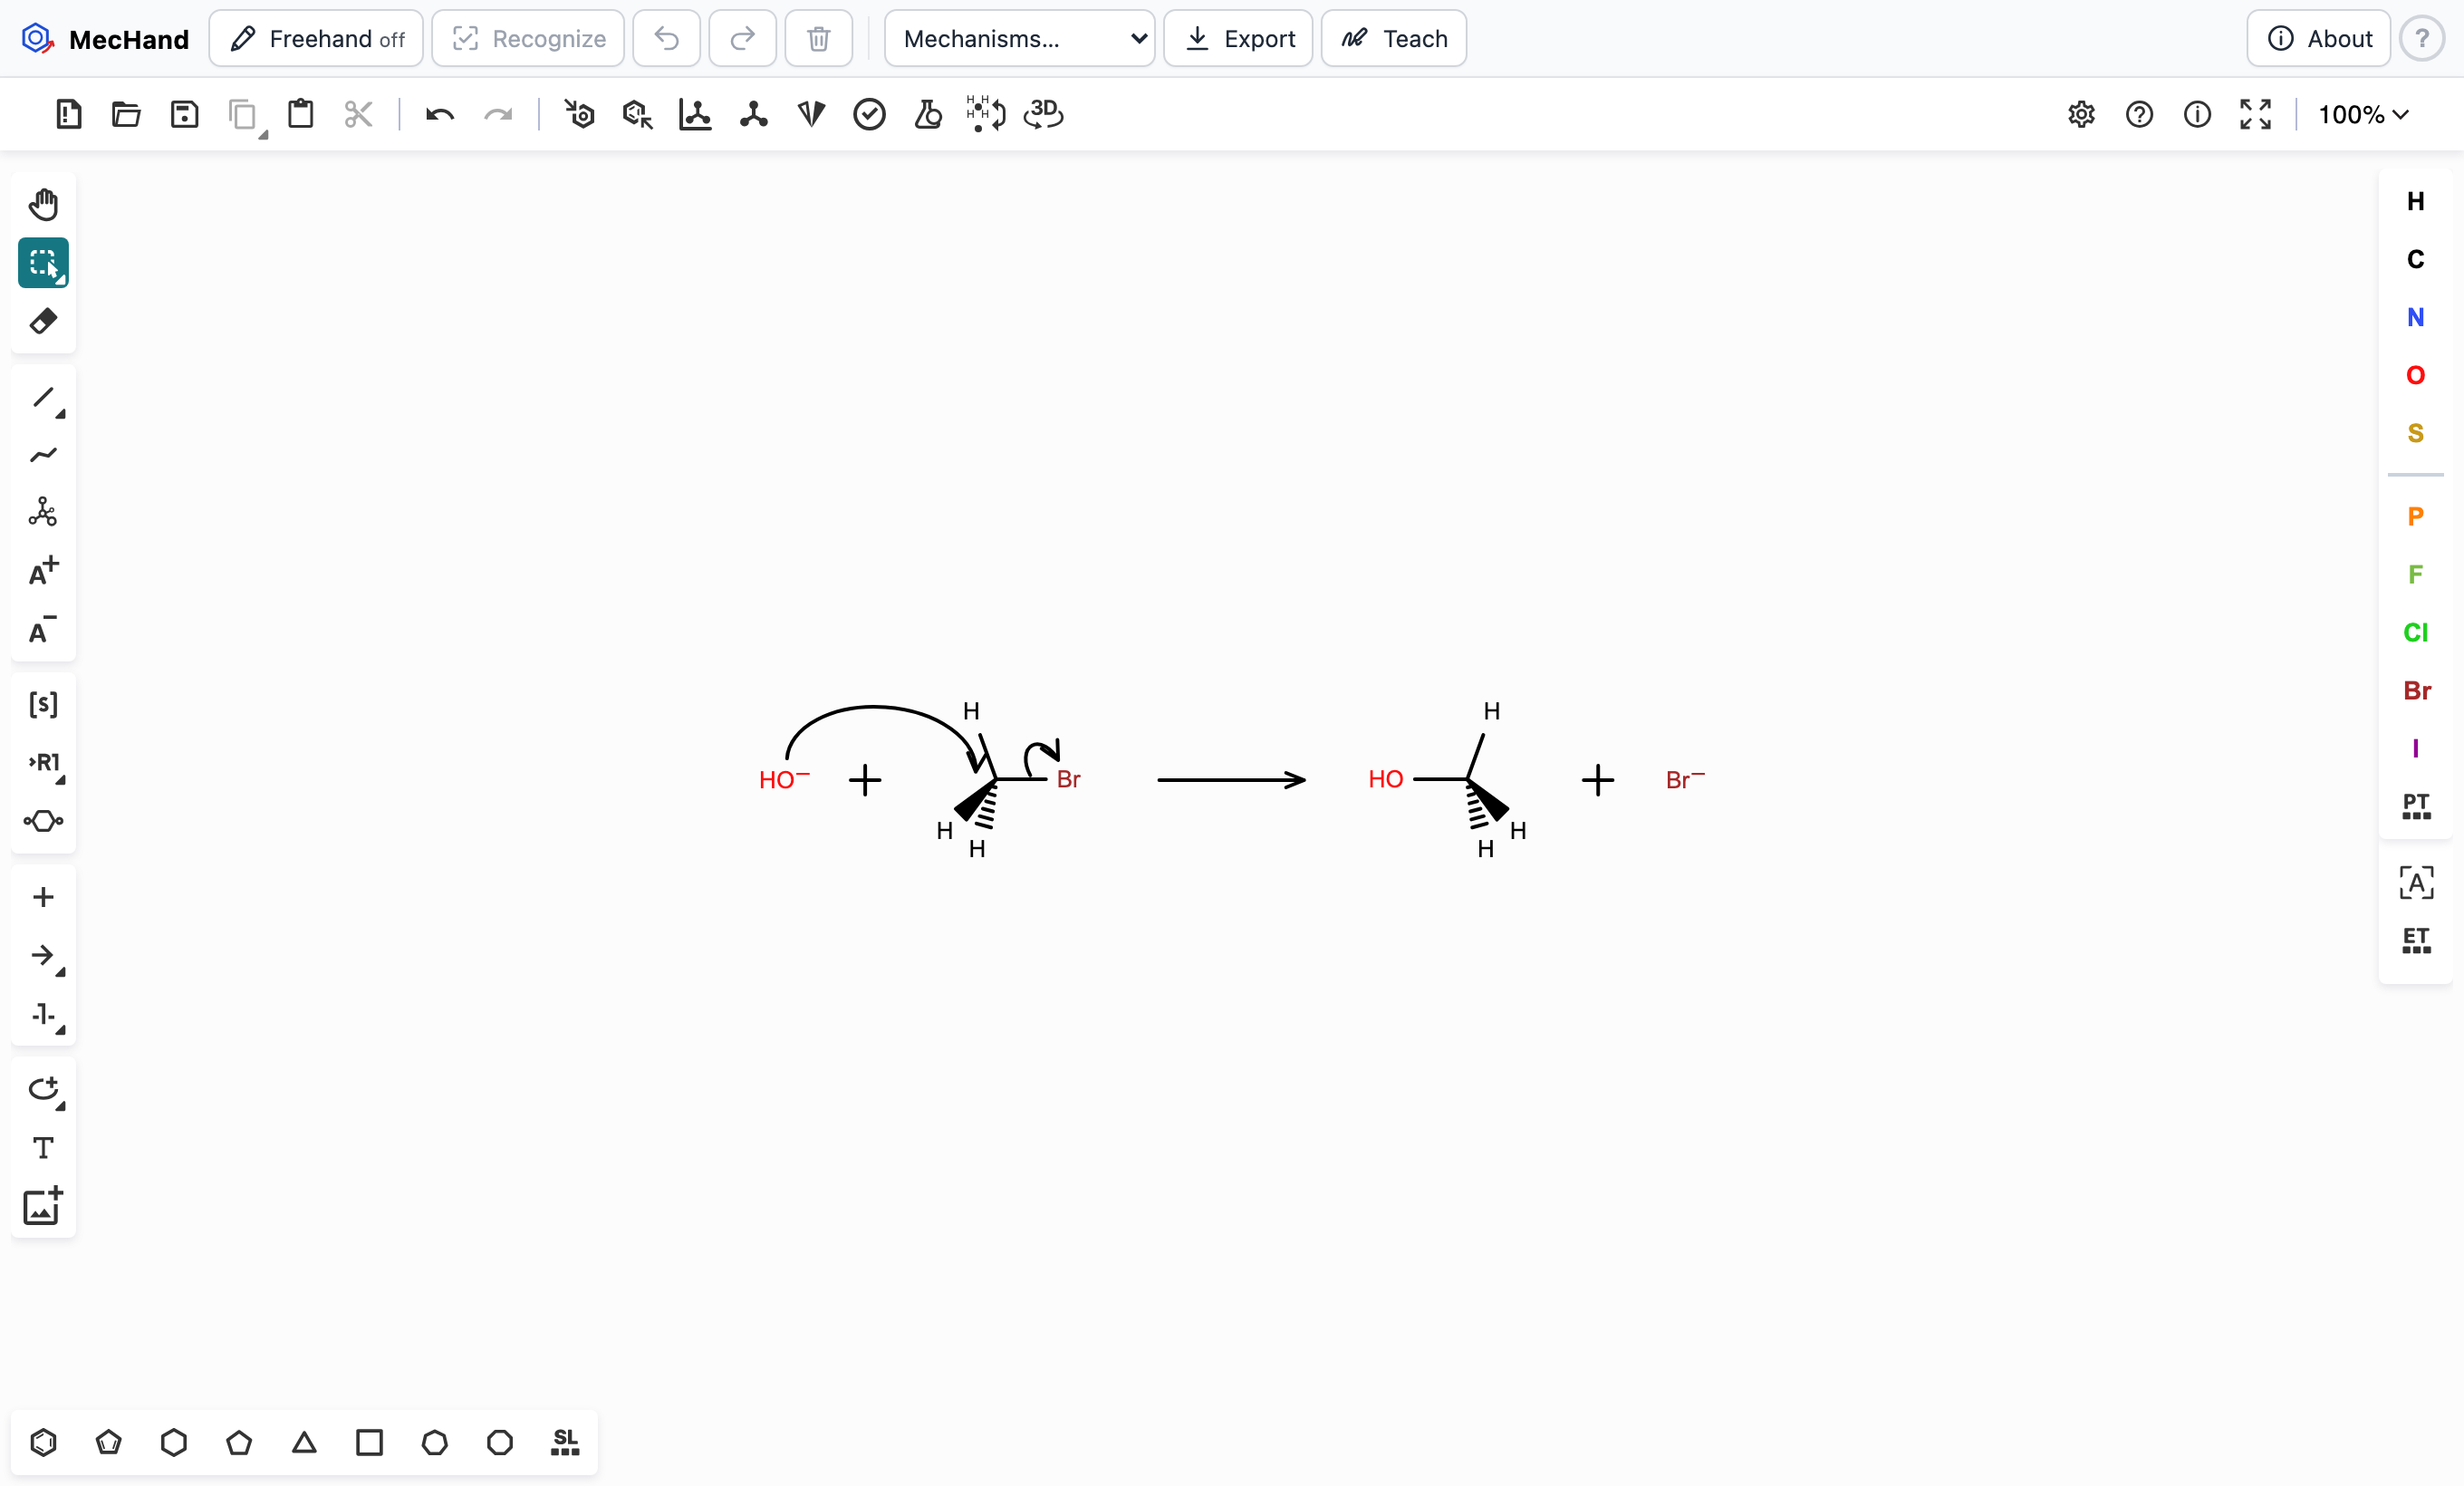
\includegraphics[width=\linewidth]{app-template.png}
  \caption{MecHand with the S\textsubscript{N}2 template open. The MecHand bar is at the top;
    below it is the Ketcher editor with its own toolbars.}
  \label{fig:app}
\end{figure}

The MecHand bar (Figure~\ref{fig:app}) has these controls:

\begin{center}
\begin{tabularx}{\linewidth}{@{}lX@{}}
  \toprule
  Control & Purpose \\
  \midrule
  \btn{Freehand} \key{Alt/Option F} & Turns the pen layer on and off. When it is off, Ketcher's tools work as usual. \\
  \btn{Recognize} \key{Space} & Reads your ink and shows what MecHand understood. \\
  \btn{Undo ink}, \btn{Clear ink} & Remove the last stroke, or all strokes not yet inserted. \\
  \btn{Templates\ldots} & Opens one of 13 standard mechanisms. \\
  \btn{Export} & TikZ, chemfig, ChemDraw (CDXML), MOL/RXN, KET or SMILES. \\
  \btn{Teach} & Teaches MecHand your handwriting. \\
  \btn{About}, \btn{?} & Recognition details and browser notes; help labels on every button. \\
  \bottomrule
\end{tabularx}
\end{center}

\paragraph{Running it on your own computer (optional).}
Install Node.js (on macOS: \texttt{brew install node}; elsewhere, the installer from
\url{https://nodejs.org}), then run \texttt{npm ci} and \texttt{npm run dev} in the
\texttt{ketcher-mechhand} folder of the repository and open \url{http://localhost:5173}.

%% ─────────────────────────────────────────────────────────────────────────────
\section{Your first mechanism: S\textsubscript{N}2}

We will draw the reactants of the S\textsubscript{N}2 reaction of hydroxide with bromomethane,
with its two curved arrows:

\begin{center}
  % Generated by MecHand (npm run export:figures) from template "sn2". Do not edit.
% MecHand TikZ export: 1 Ketcher unit = 0.8 cm; needs \usetikzlibrary{arrows.meta,bending}
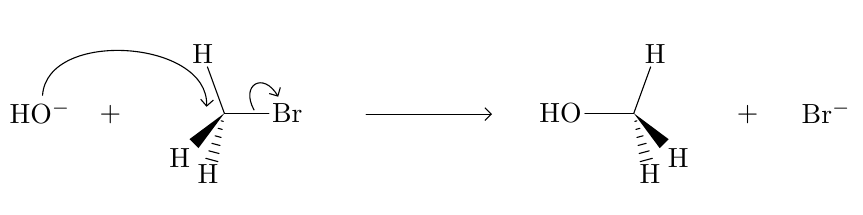
\begin{tikzpicture}[line cap=round, line join=round]
  % atoms
  \node[inner sep=1pt] (a0) at (0,0.762) {\smash{\llap{H}}O\smash{\rlap{$^{-}$}}};
  \coordinate (a1) at (2.326,0.773);
  \node[inner sep=1pt] (a2) at (3.126,0.773) {Br};
  \node[inner sep=1pt] (a3) at (2.052,1.524) {H};
  \node[inner sep=1pt] (a4) at (1.76,0.207) {H};
  \node[inner sep=1pt] (a5) at (2.119,0) {H};
  \coordinate (a6) at (7.526,0.773);
  \node[inner sep=1pt] (a7) at (6.726,0.773) {\smash{\llap{H}}O};
  \node[inner sep=1pt] (a8) at (7.799,1.524) {H};
  \node[inner sep=1pt] (a9) at (8.091,0.207) {H};
  \node[inner sep=1pt] (a10) at (7.733,0) {H};
  \node[inner sep=1pt] (a11) at (9.851,0.762) {Br\smash{\rlap{$^{-}$}}};
  % bonds
  \draw (a1) -- (a2);
  \draw (a1) -- (a3);
  \fill (2.326,0.773) -- (1.997,0.33) -- (1.883,0.444) -- cycle;
  \draw (2.312,0.67) -- (2.286,0.677) (2.299,0.568) -- (2.247,0.582) (2.285,0.466) -- (2.208,0.487) (2.271,0.364) -- (2.168,0.391) (2.258,0.262) -- (2.129,0.296) (2.244,0.159) -- (2.09,0.201);
  \draw (a6) -- (a7);
  \draw (a6) -- (a8);
  \fill (7.526,0.773) -- (7.968,0.444) -- (7.855,0.33) -- cycle;
  \draw (7.565,0.677) -- (7.539,0.67) (7.604,0.582) -- (7.553,0.568) (7.644,0.487) -- (7.566,0.466) (7.683,0.391) -- (7.58,0.364) (7.722,0.296) -- (7.594,0.262) (7.762,0.201) -- (7.607,0.159);
  % pluses
  \node at (0.88,0.762) {$+$};
  \node at (8.971,0.762) {$+$};
  % arrows
  \draw[-{Straight Barb}] (4.126,0.762) -- (5.726,0.762);
  \draw[-{Straight Barb}] (0.017,1.002) .. controls (0.077,1.853) and (2.16,1.706) .. (2.1,0.855);
  \draw[-{Straight Barb}] (2.703,0.815) .. controls (2.523,1.142) and (2.831,1.311) .. (3.01,0.983);
\end{tikzpicture}

\end{center}

\begin{enumerate}[leftmargin=*]
  \item Press \btn{Freehand} (or \key{Alt/Option F}). The canvas turns faintly blue: you are drawing ink.
  \item Write \textbf{O} with a small \textbf{$-$} up and to its right: hydroxide.
  \item Write a \textbf{$+$}, then draw the carbon: three short lines ending at three \textbf{H}
    and one line ending at \textbf{Br}. Leave a small gap between each line and its letter, as
    in a printed formula, and make the lines about two or three times longer than the letters are tall.
  \item Draw the first curved arrow from the oxygen to the carbon, and finish it with a
    \emph{full} arrowhead --- a small ``V'', drawn without lifting the pen or as a separate stroke.
  \item Draw the second curved arrow from the middle of the C--Br bond to the bromine.
\end{enumerate}

\begin{figure}[h]
  \centering
  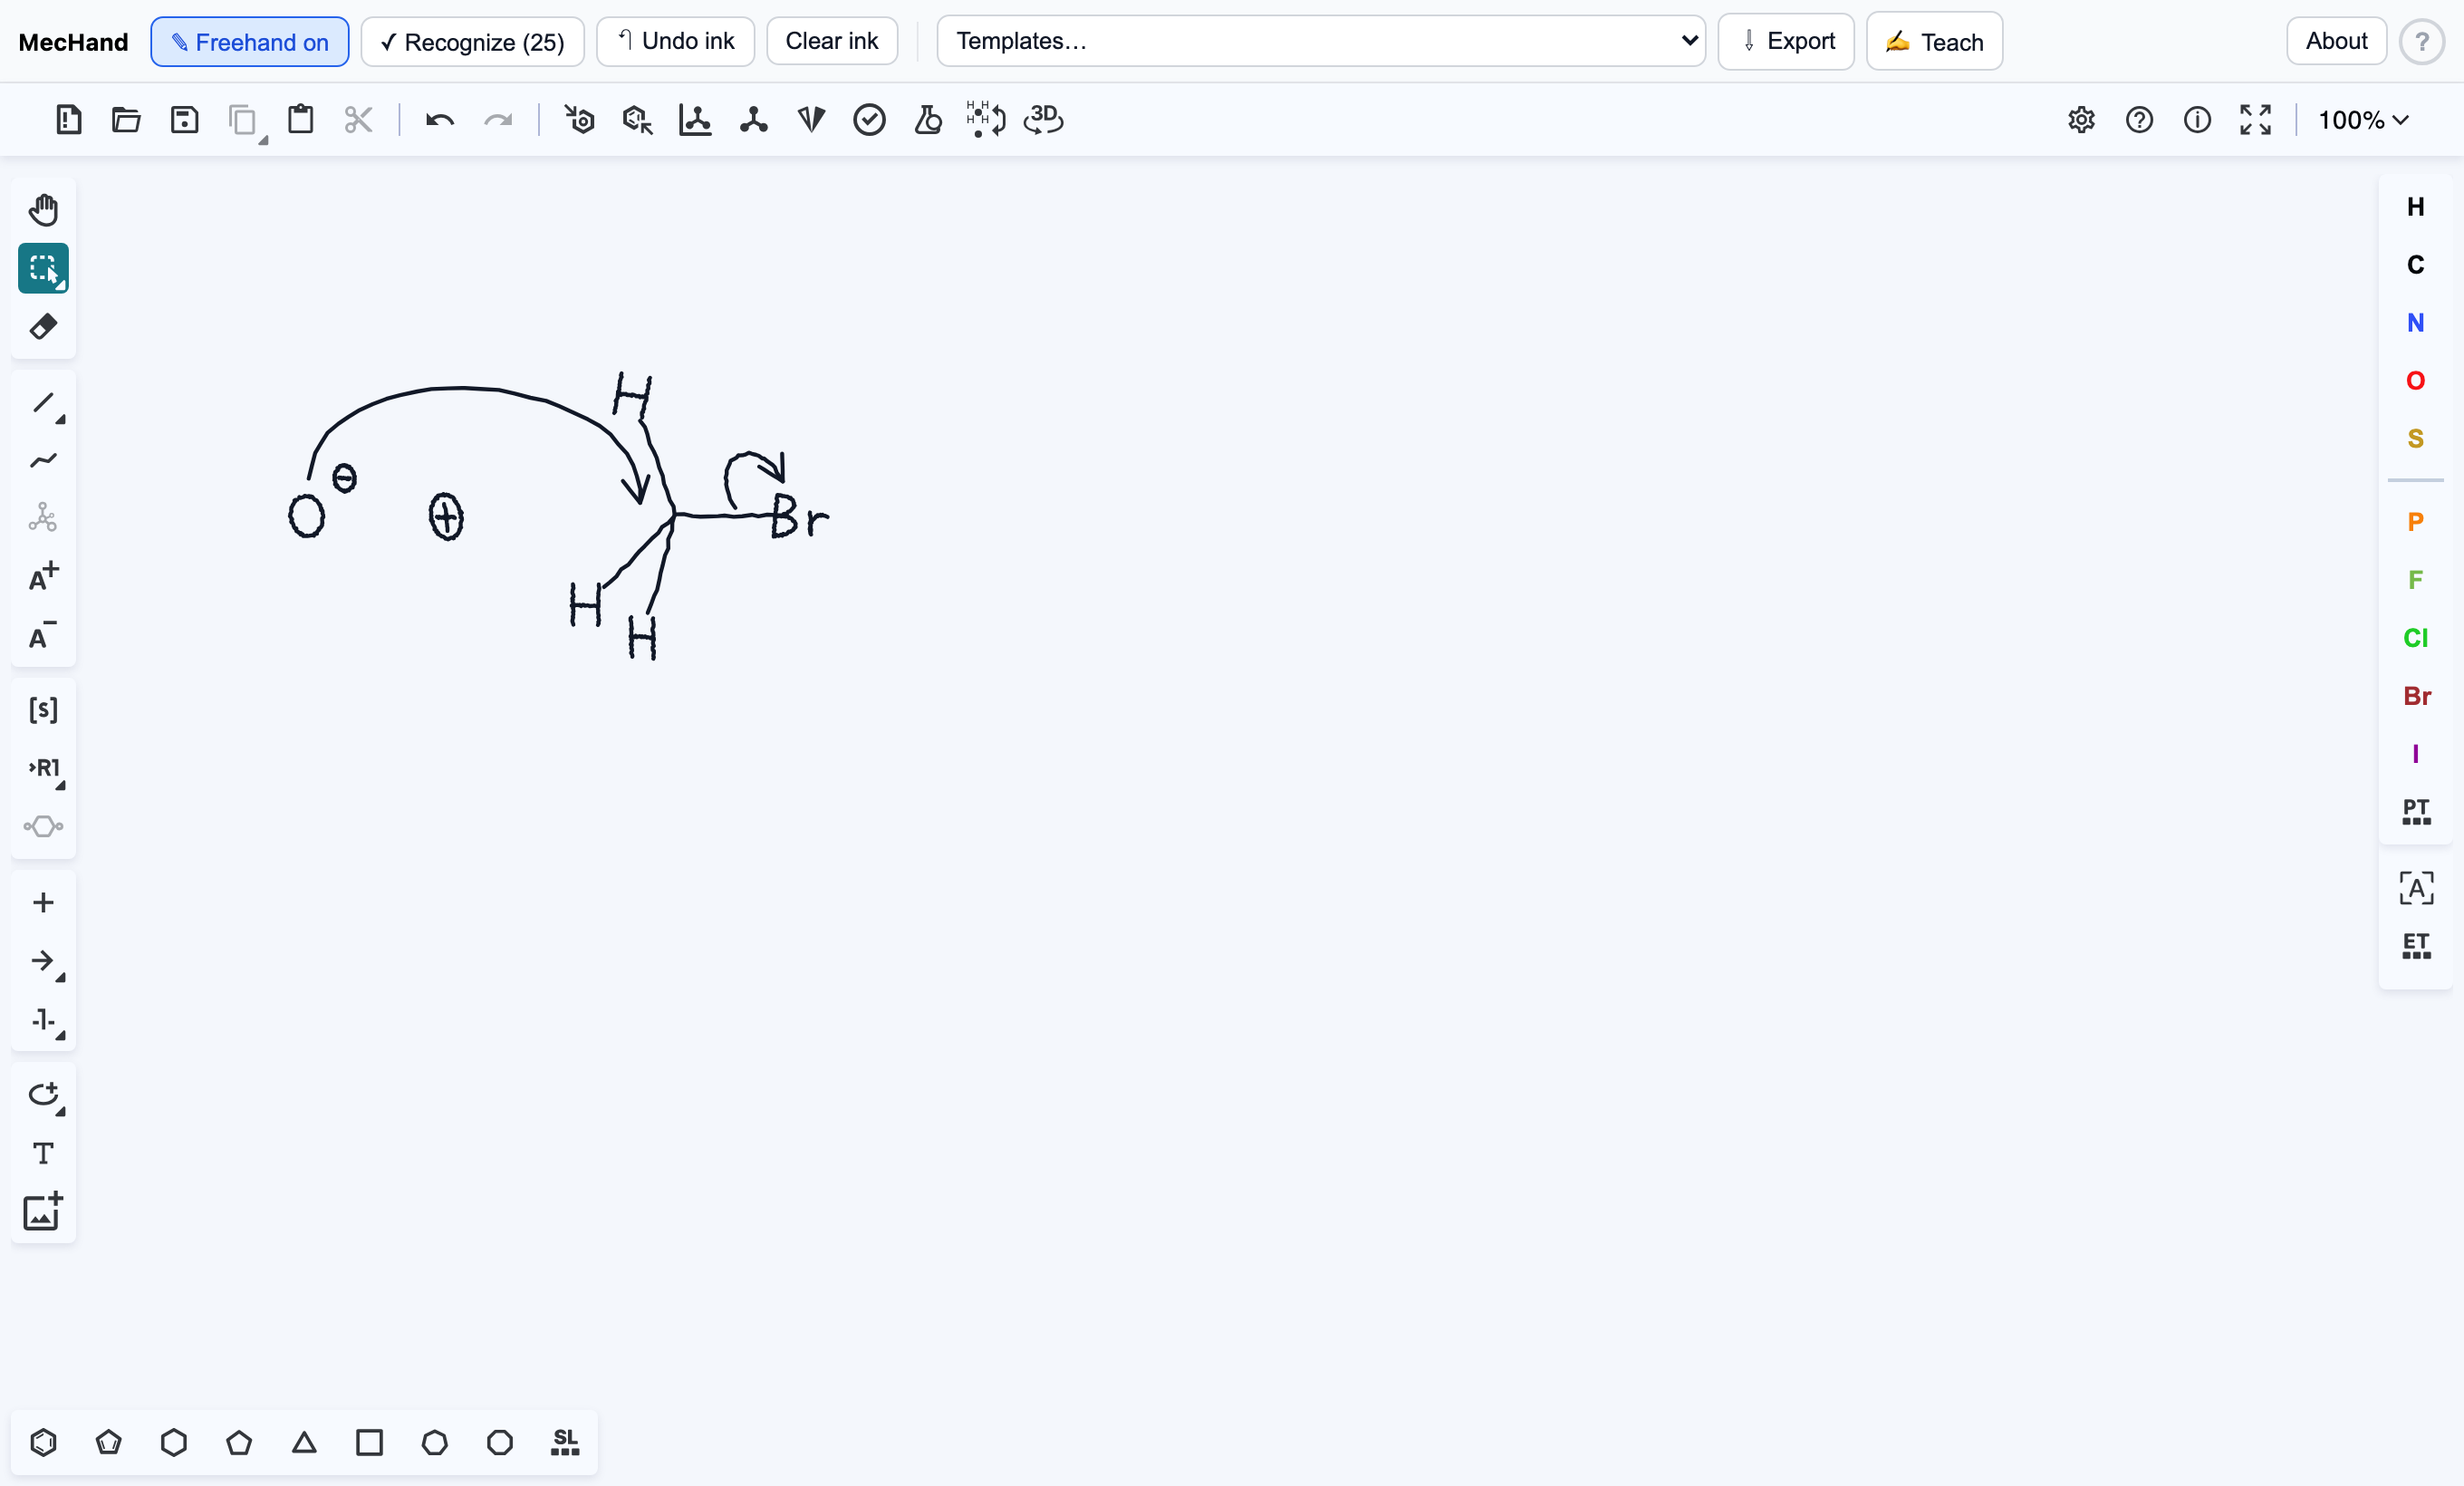
\includegraphics[width=0.9\linewidth]{freehand-ink.png}
  \caption{The S\textsubscript{N}2 reactants drawn as ink.}
  \label{fig:ink}
\end{figure}

Now press \btn{Recognize} (or \key{Space}).

%% ─────────────────────────────────────────────────────────────────────────────
\section{Is this what you meant?}

MecHand colours your ink by how it read each stroke --- \textcolor{blue!70!black}{blue} bonds,
\textcolor{green!45!black}{green} labels, \textcolor{red!70!black}{red} arrows,
\textcolor{gray}{grey} not understood --- and shows a clean drawing of the result with its confidence
(Figure~\ref{fig:dialog}).

\begin{figure}[h]
  \centering
  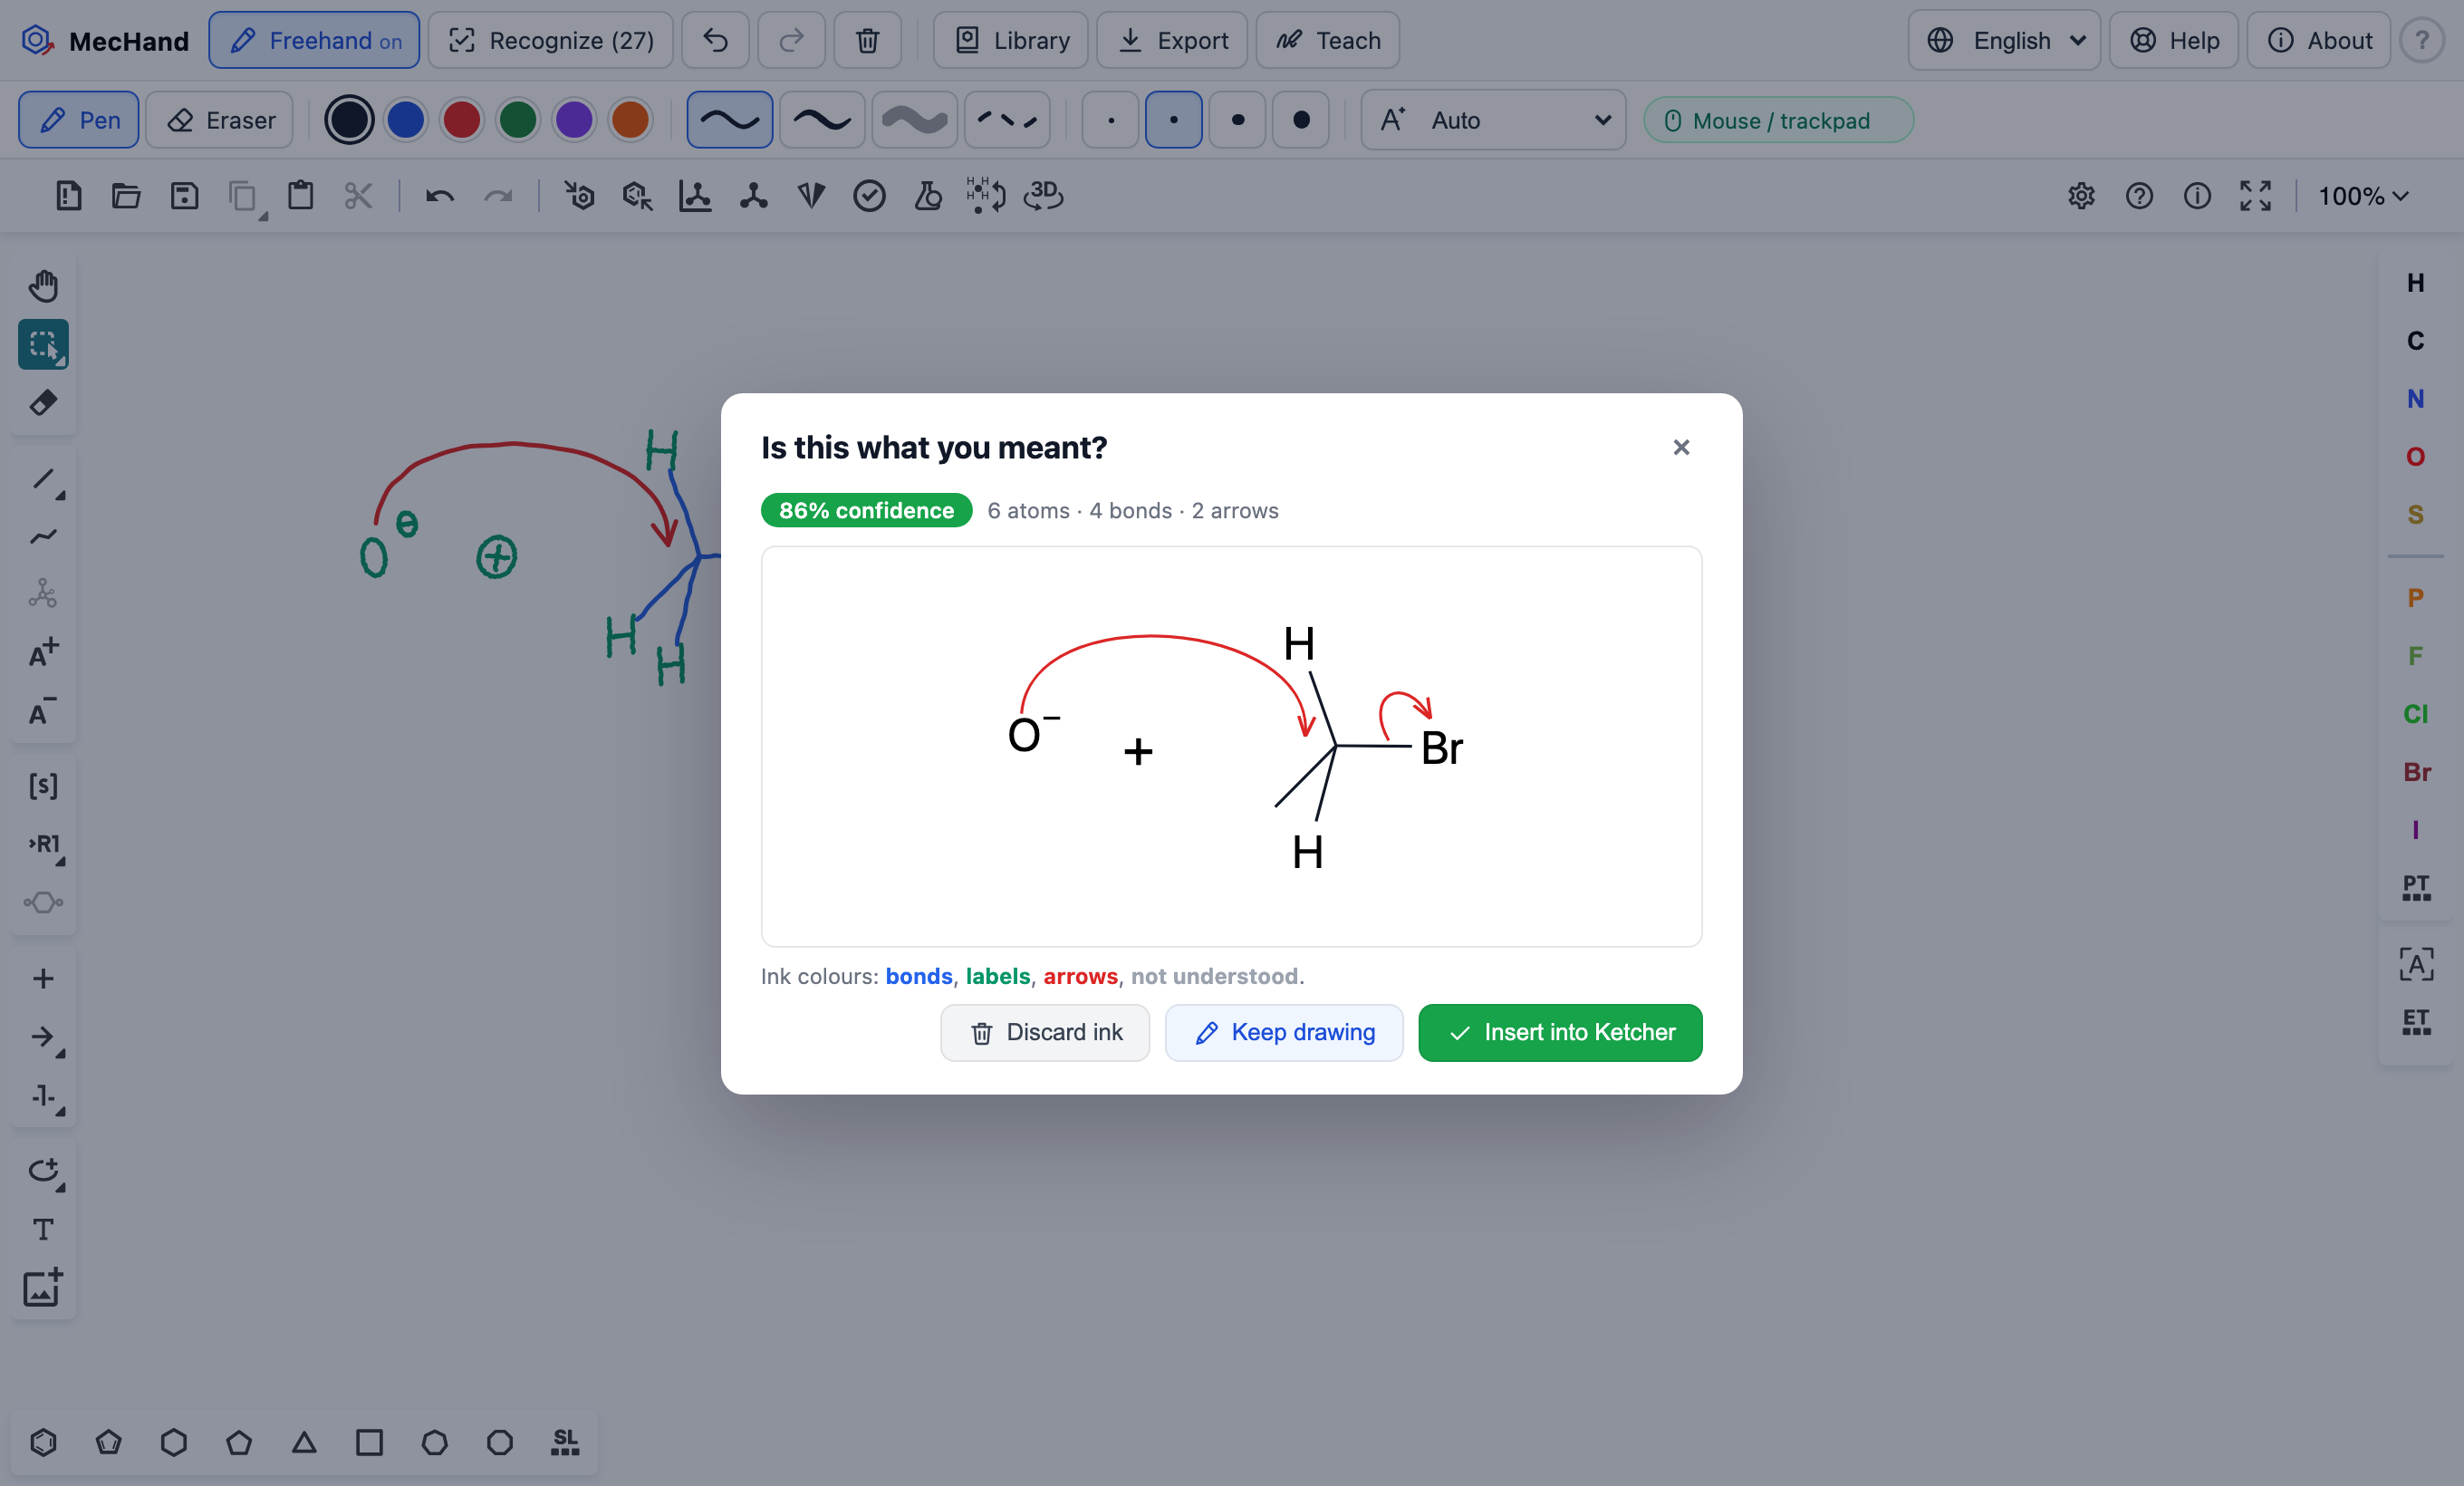
\includegraphics[width=0.9\linewidth]{recognize-dialog.png}
  \caption{The recognition dialog: 6 atoms, 4 bonds and 2 arrows, with 87\,\% confidence.}
  \label{fig:dialog}
\end{figure}

\begin{description}[leftmargin=*]
  \item[\btn{Insert into Ketcher}] adds the structure and the arrows to the canvas. They are now
    ordinary Ketcher objects: move them, add stereochemistry, or keep drawing with Ketcher's tools.
  \item[\btn{Keep drawing}] closes the dialog and keeps the ink, so you can fix or add strokes.
  \item[\btn{Discard ink}] deletes the strokes.
\end{description}

\paragraph{Electron-flow check.} Each curved arrow is attached to the atom or bond nearest to its
ends. The dialog warns you when an electron-pair arrow starts at an atom with no lone pair (start it
at a lone pair or at a bond instead), when an arrow starts or ends on nothing, or when an arrow would
give C, N, O or F more than an octet while no bond to that atom breaks in the same step. Try it:
draw an arrow from the CH\textsubscript{3} carbon to the oxygen and recognize again.

\subsection*{What MecHand understands}

\begin{center}
\begin{tabularx}{\linewidth}{@{}lX@{}}
  \toprule
  You draw & MecHand reads \\
  \midrule
  a line; a zig-zag or polygon in one stroke & bonds; a chain or a ring \\
  two or three close parallel lines & a double or triple bond \\
  letters & atom labels: C, H, N, O, S, P, F, Cl, Br, I, B, Si, Li, Na, K, Mg, Al, Fe, Cu, Zn, Pt, Pd\ldots \\
  $+$, $-$, $\oplus$, $\ominus$, $2-$, $3+$ at the upper right of an atom & a formal charge \\
  a single dot next to an atom & a radical \\
  a $+$ between molecules & a reaction plus sign \\
  a curve with a full head / a single barb & an electron-pair / a single-electron arrow \\
  a long straight arrow & a reaction arrow \\
  \bottomrule
\end{tabularx}
\end{center}

%% ─────────────────────────────────────────────────────────────────────────────
\section{Templates: practise with standard mechanisms}

\btn{Templates\ldots} opens 13 textbook mechanisms: S\textsubscript{N}2, E2, addition to a carbonyl,
aromatic nitration, Diels--Alder and Cl\textsubscript{2} homolysis (organic); the NH\textsubscript{3}--BF\textsubscript{3}
Lewis adduct, associative substitution at Pt(II), hydrolysis of SiCl\textsubscript{4} and the acidity of
[Fe(OH\textsubscript{2})\textsubscript{6}]\textsuperscript{3+} (inorganic); and serine-protease acylation,
alcohol dehydrogenase and a kinase (biochemistry). A good exercise: open a template, study it, clear
the canvas, and redraw it by hand. The Diels--Alder template, as exported to TikZ:

\begin{center}
  % Generated by MecHand (npm run export:figures) from template "diels_alder". Do not edit.
% MecHand TikZ export: 1 Ketcher unit = 0.8 cm; needs \usetikzlibrary{arrows.meta,bending}
\begin{tikzpicture}[line cap=round, line join=round]
  % atoms
  \coordinate (a0) at (0.79,1.6);
  \coordinate (a1) at (0.097,1.2);
  \coordinate (a2) at (0.097,0.4);
  \coordinate (a3) at (0.79,0);
  \coordinate (a4) at (1.99,1.2);
  \coordinate (a5) at (1.99,0.4);
  \coordinate (a6) at (5.883,1.6);
  \coordinate (a7) at (5.19,1.2);
  \coordinate (a8) at (5.19,0.4);
  \coordinate (a9) at (5.883,0);
  \coordinate (a10) at (6.576,0.4);
  \coordinate (a11) at (6.576,1.2);
  % bonds
  \draw (a0) -- (a1);
  \draw[transform canvas={xshift=0.06cm,yshift=-0.104cm}, shorten <=0.096cm, shorten >=0.096cm] (a0) -- (a1);
  \draw (a1) -- (a2);
  \draw (a2) -- (a3);
  \draw[transform canvas={xshift=0.06cm,yshift=0.104cm}, shorten <=0.096cm, shorten >=0.096cm] (a2) -- (a3);
  \draw[transform canvas={xshift=0.06cm,yshift=0cm}] (a4) -- (a5);
  \draw[transform canvas={xshift=-0.06cm,yshift=0cm}] (a4) -- (a5);
  \draw (a6) -- (a7);
  \draw (a7) -- (a8);
  \draw[transform canvas={xshift=0.12cm,yshift=0cm}, shorten <=0.096cm, shorten >=0.096cm] (a7) -- (a8);
  \draw (a8) -- (a9);
  \draw (a9) -- (a10);
  \draw (a10) -- (a11);
  \draw (a11) -- (a6);
  % arrows
  \draw[-{Straight Barb}] (2.79,0.8) -- (4.39,0.8);
  \draw[-{Straight Barb}] (0.444,1.448) .. controls (0.448,2.177) and (1.995,2.169) .. (1.991,1.44);
  \draw[-{Straight Barb}] (1.968,0.843) .. controls (1.671,1.435) and (0.468,0.831) .. (0.765,0.239);
  \draw[-{Straight Barb}] (0.405,0.172) .. controls (0.046,-0.088) and (-0.359,0.469) .. (0,0.73);
\end{tikzpicture}

\end{center}

%% ─────────────────────────────────────────────────────────────────────────────
\section{Exporting to \LaTeX{}}

\btn{Export} converts everything on the canvas --- including curved arrows --- into code
(Figure~\ref{fig:export}). \textbf{TikZ} gives absolute coordinates and Bézier arrows that are easy to
adjust; \textbf{chemfig} gives a reaction scheme with \verb|\chemmove| arrows. Copy the code, or
download it, and paste it into your document together with the preamble lines shown at the top:

\begin{verbatim}
\usepackage{tikz}
\usetikzlibrary{arrows.meta,bending}
\usepackage{chemfig}                       % for the chemfig export
\usetikzlibrary{calc}                      % (chemfig arrows)
\end{verbatim}

\begin{figure}[h]
  \centering
  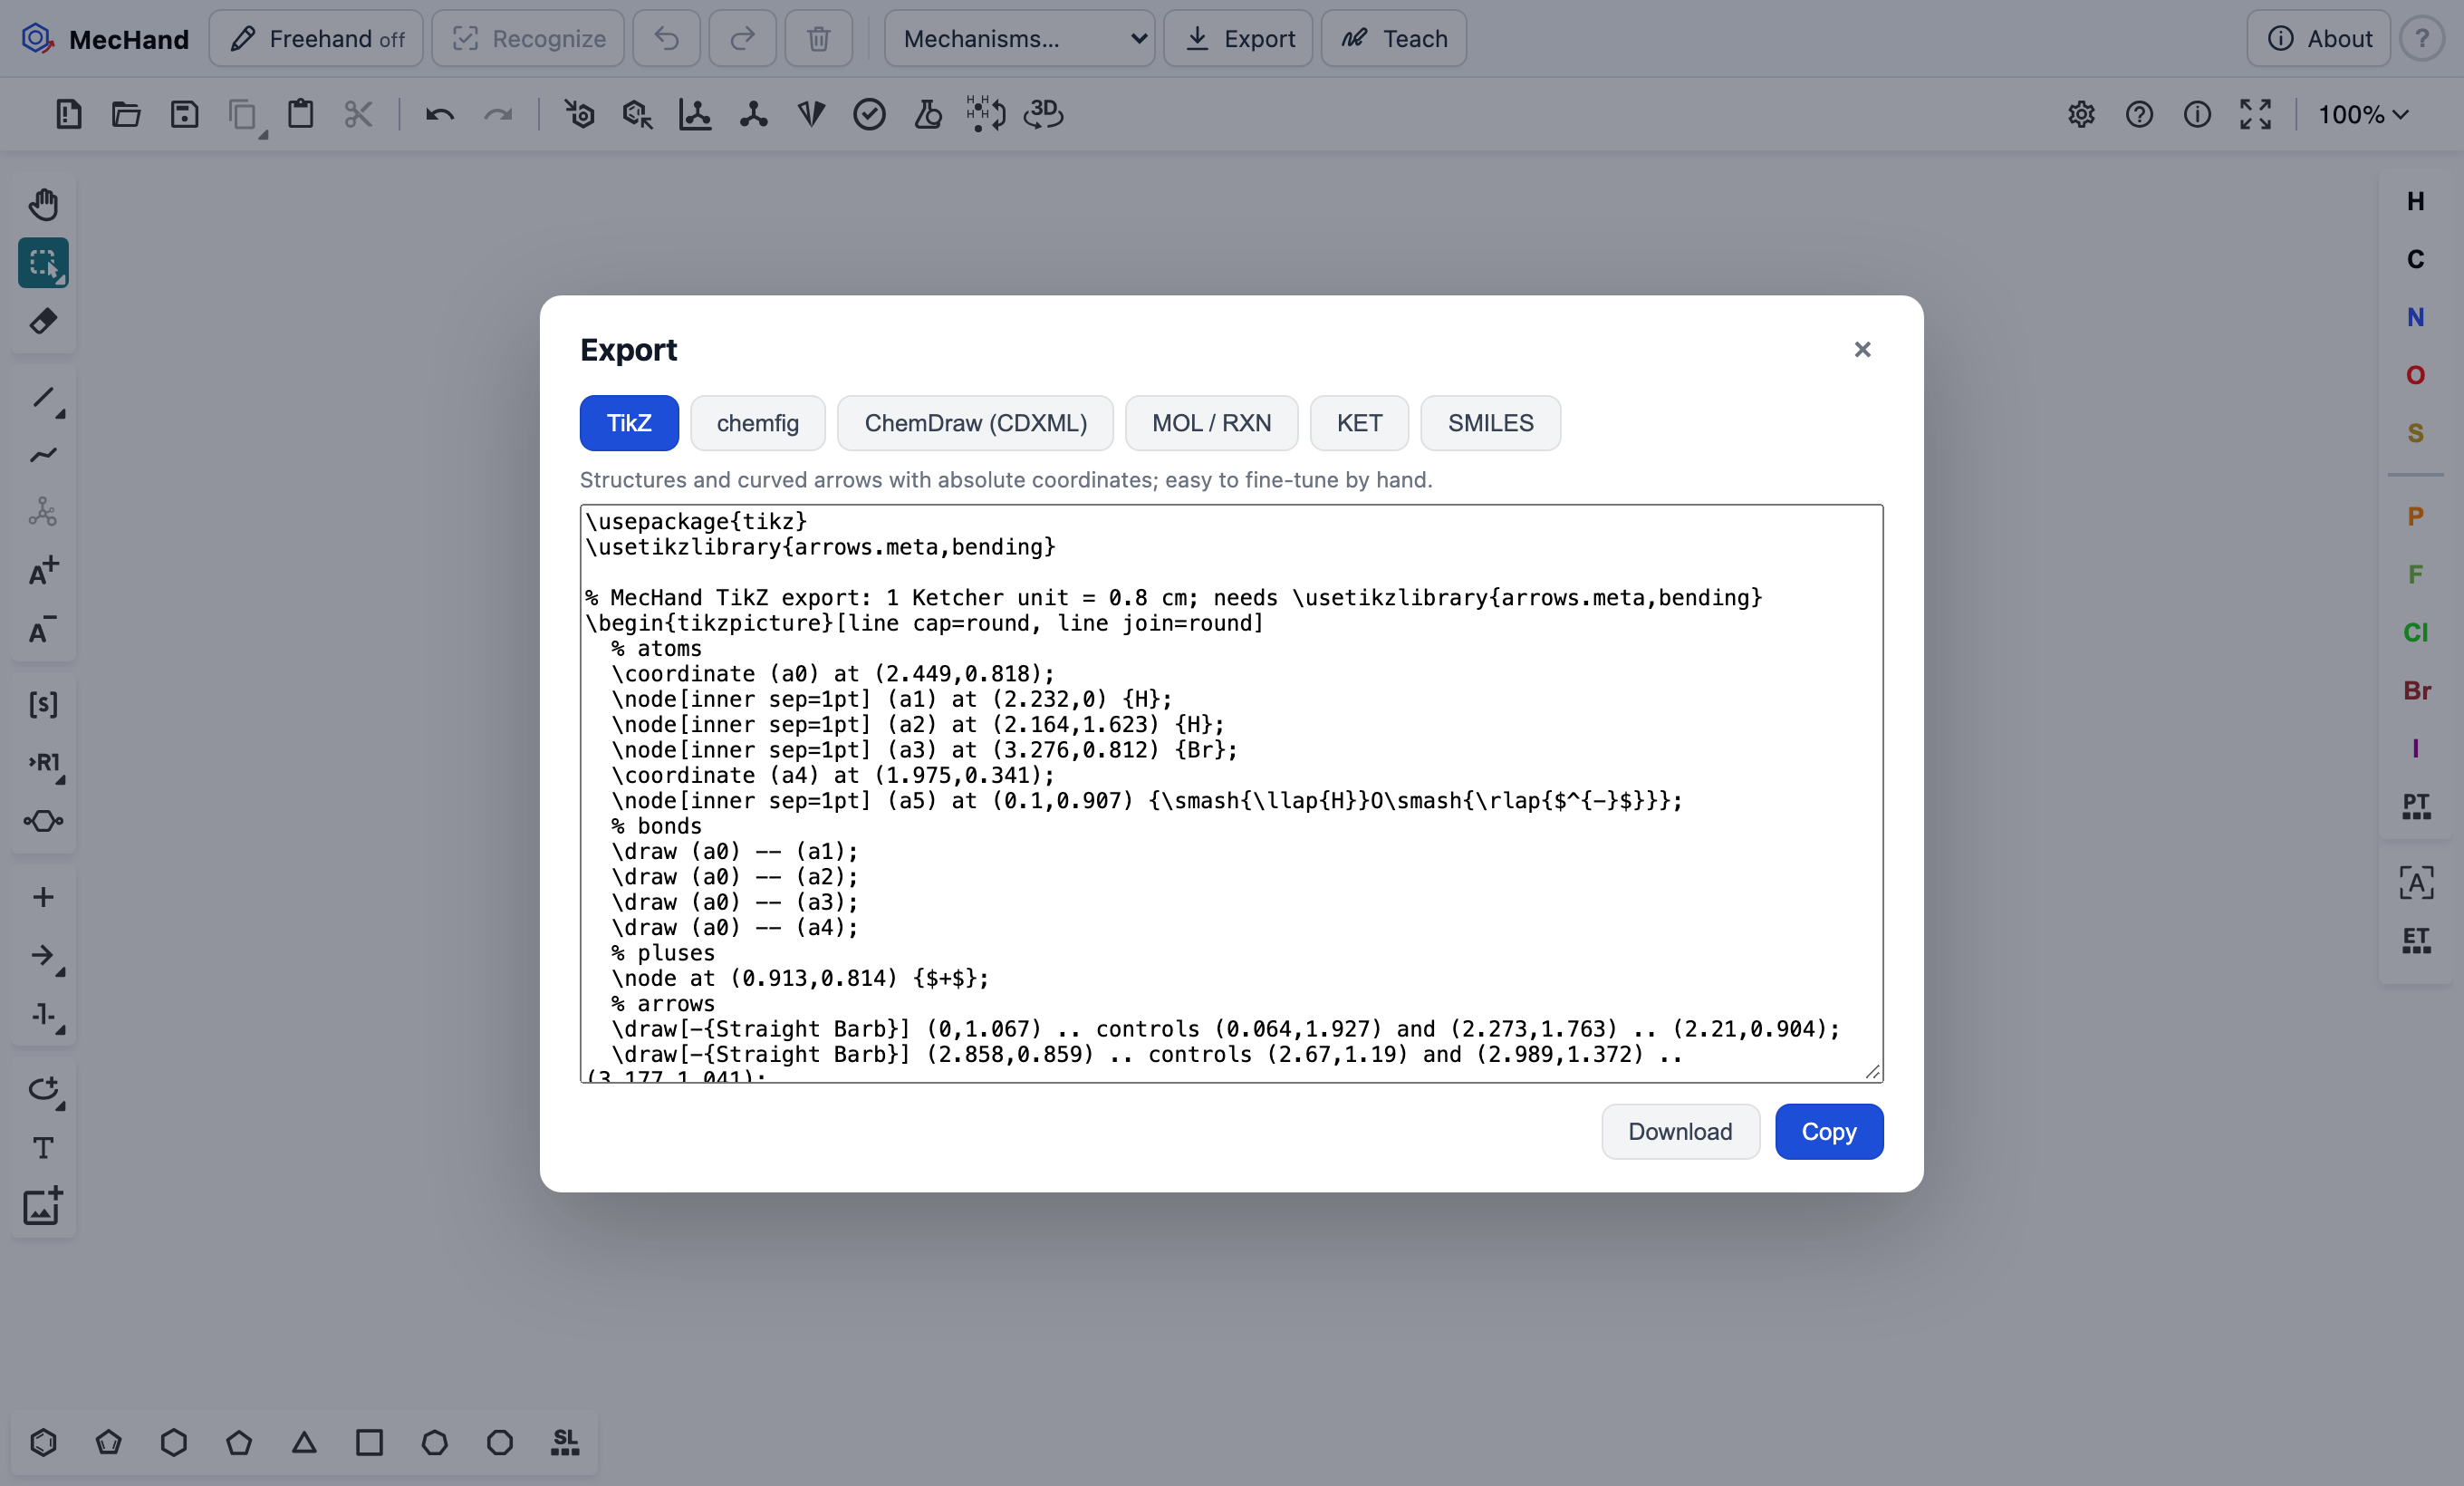
\includegraphics[width=0.9\linewidth]{export-dialog.png}
  \caption{The Export dialog with the TikZ code of the Diels--Alder template.}
  \label{fig:export}
\end{figure}

The figures in this tutorial were produced exactly this way. Here is the homolysis of
Cl\textsubscript{2} exported to chemfig (compile twice: chemfig places the arrows using positions
recorded in the first run):

\begin{center}
  % Generated by MecHand (npm run export:figures) from template "radical_homolysis". Do not edit.
% MecHand chemfig export; needs \usepackage{chemfig} and \usetikzlibrary{arrows.meta,bending,calc}; compile twice for the \chemmove arrows
\schemestart
  \chemfig{@{a0}Cl-[:0]@{a1}Cl}
  \arrow{->}
  \chemfig{\charge{90=\.}{Cl}}
  \+
  \chemfig{\charge{90=\.}{Cl}}
\schemestop
\chemmove{
  \draw[-{Straight Barb[harpoon,swap]}, shorten <=2pt, shorten >=2pt] ($(a0)!0.5!(a1)$) .. controls +(0.46em,1.53em) and +(0.46em,1.53em) .. (a0);
  \draw[-{Straight Barb[harpoon]}, shorten <=2pt, shorten >=2pt] ($(a0)!0.5!(a1)$) .. controls +(-0.46em,1.53em) and +(-0.46em,1.53em) .. (a1);
}

\end{center}

\noindent The other formats --- CDXML, MOL/RXN, KET and SMILES --- open in ChemDraw, Marvin, RDKit and
other software. Ketcher also opens CDXML, MOL, RXN and SMILES files, so a mechanism started elsewhere
can be finished in MecHand.

%% ─────────────────────────────────────────────────────────────────────────────
\section{Teaching MecHand your handwriting}

If a letter is often misread, open \btn{Teach}, choose the symbol, write it in the box and press
\btn{Save sample}; a few samples per symbol help. Samples are stored in your browser and used at once.
\btn{Export samples} saves them as a file that can be added to MecHand's shared model, so the
recognizer improves for everybody (see the website, ``Handwriting recognition'').

\begin{figure}[h]
  \centering
  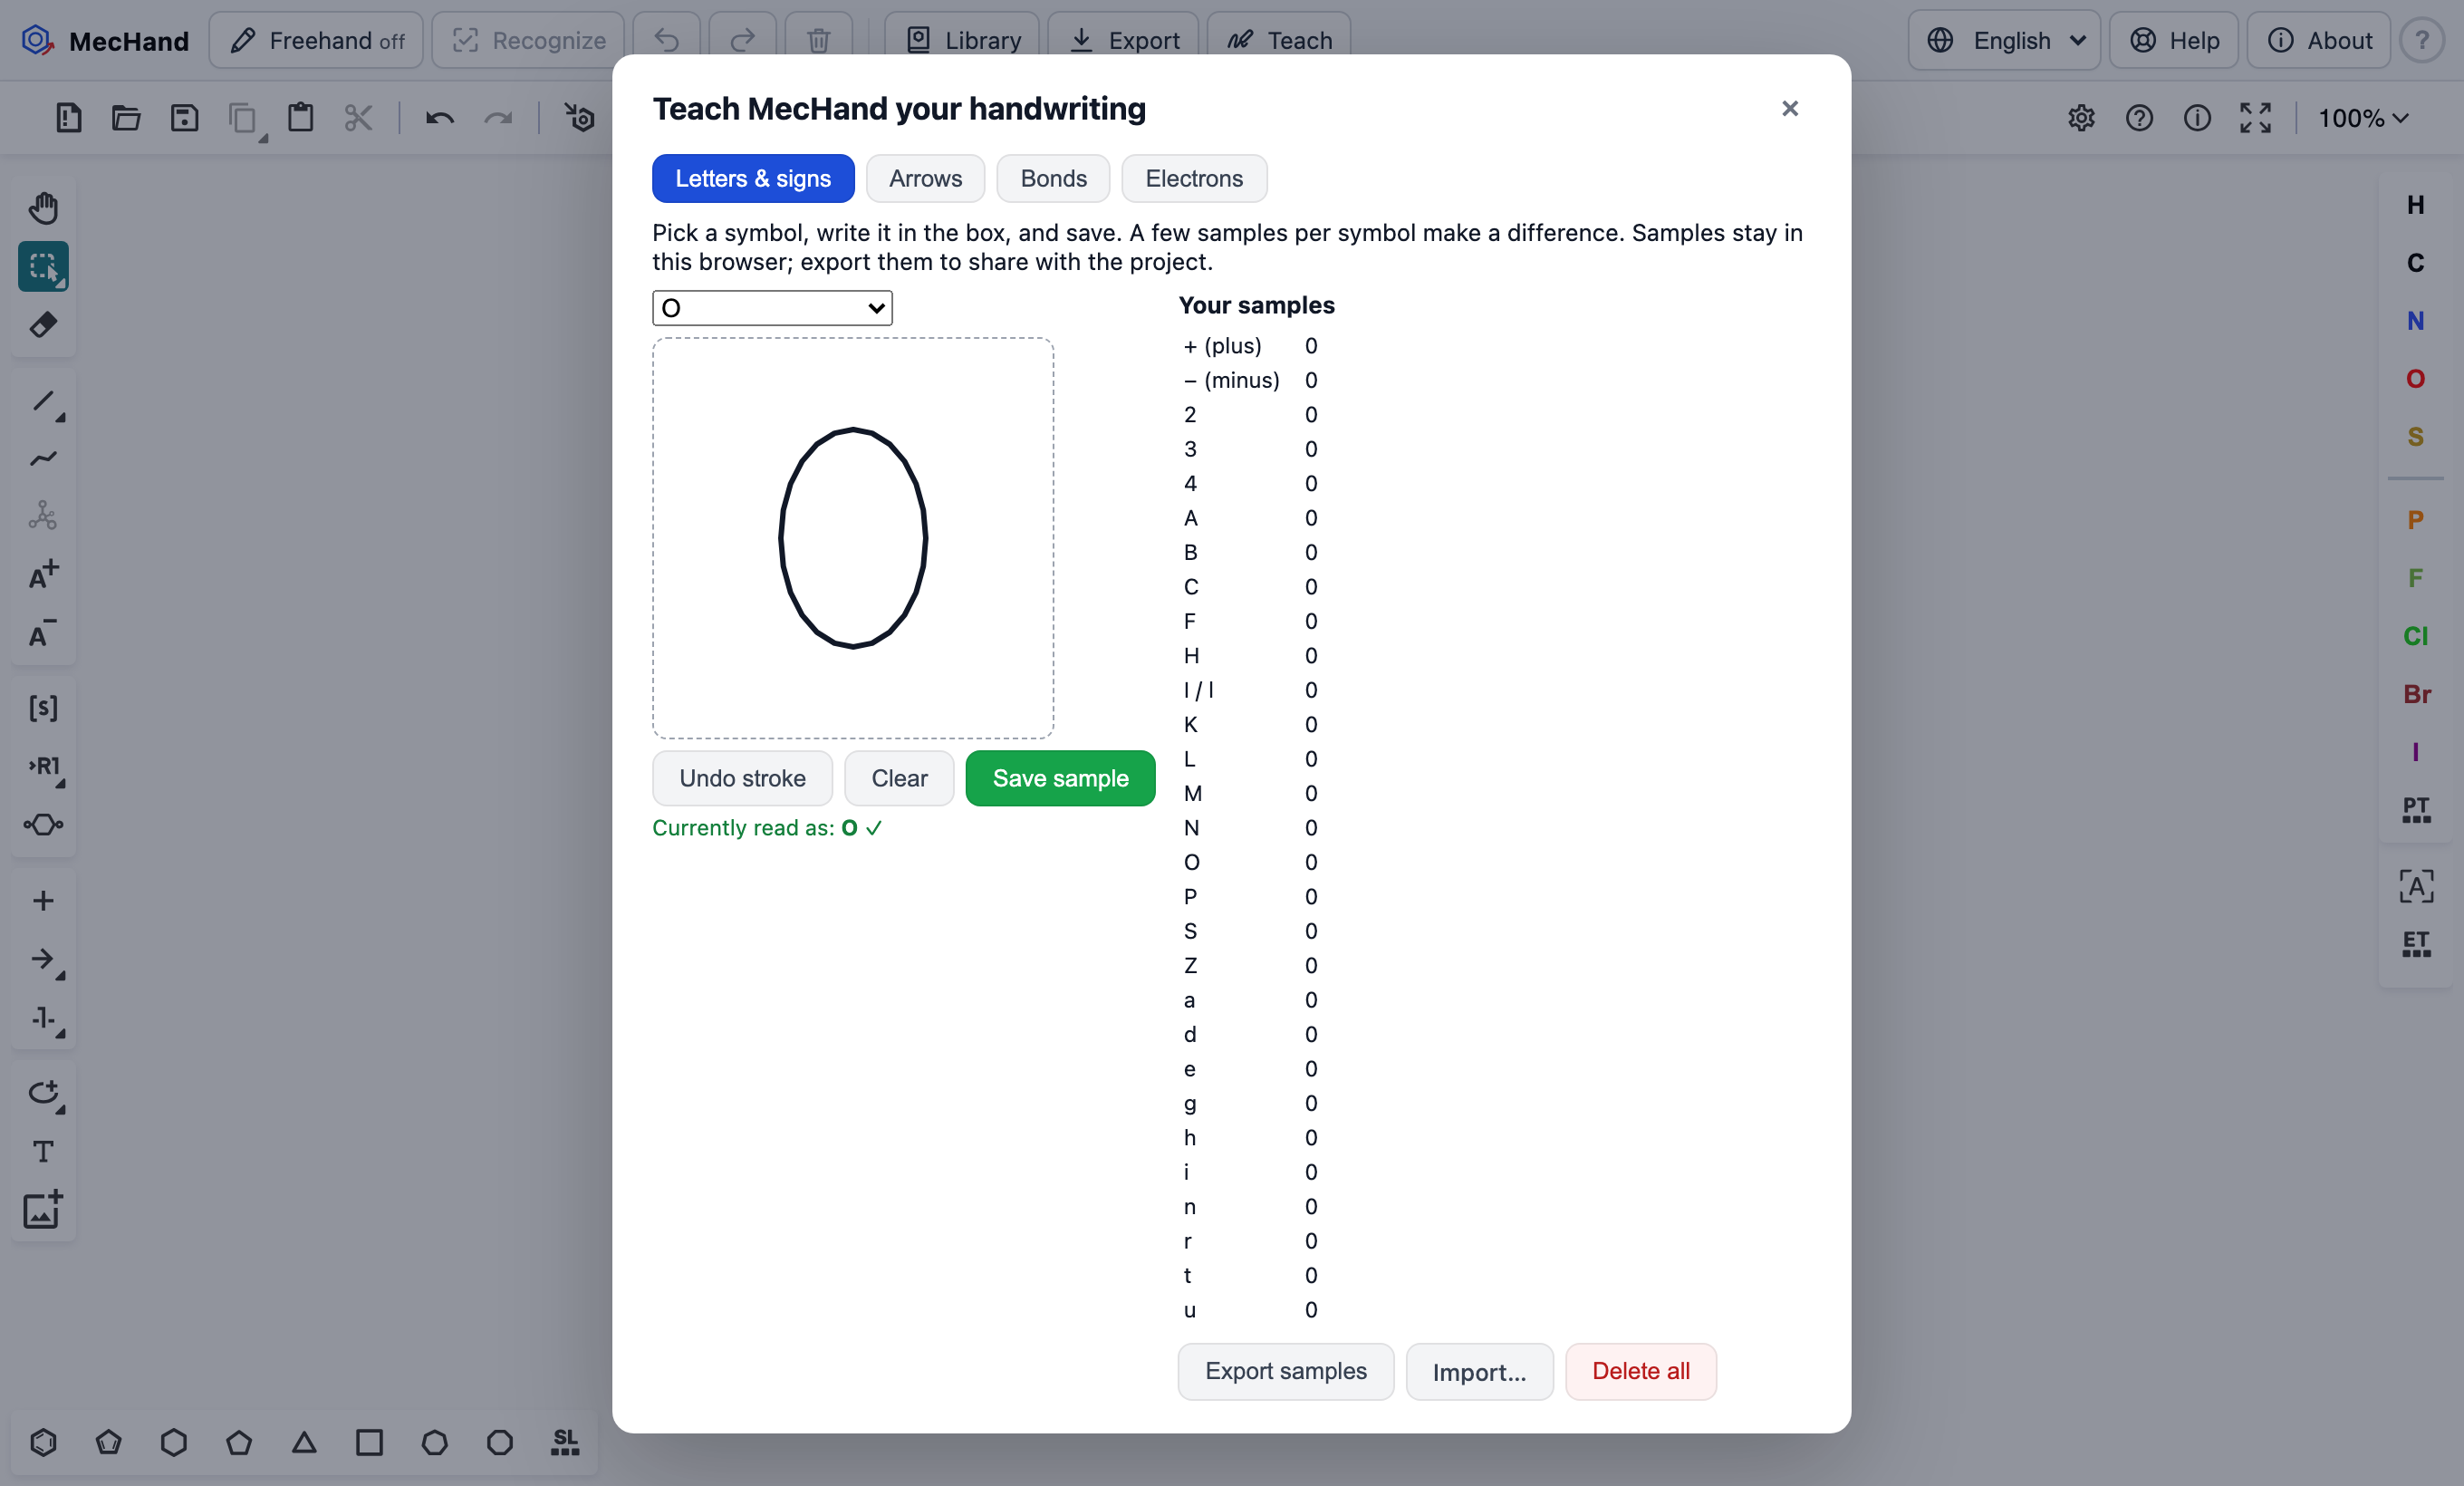
\includegraphics[width=0.75\linewidth]{teach-panel.png}
  \caption{Teach: the box shows how your sample is currently read.}
\end{figure}

%% ─────────────────────────────────────────────────────────────────────────────
\section{Tips and troubleshooting}

\begin{itemize}[leftmargin=*]
  \item \textbf{Bonds read as letters, or letters as bonds?} Draw bonds longer than letters are tall,
    and leave a small gap between a bond and its label.
  \item \textbf{An arrow is not recognized?} Make the head clearly visible: a V whose arms point back
    along the shaft. A single barb means a one-electron (fishhook) arrow.
  \item \textbf{Panning and zooming} the canvas with touch or pen only works with freehand mode off.
  \item \textbf{Undo:} in freehand mode \key{Ctrl/Cmd Z} removes the last stroke; otherwise it is
    Ketcher's undo.
  \item \textbf{Browsers:} current Chrome, Edge, Firefox and Safari, on computers and tablets (with
    Apple Pencil, S Pen and other styluses). Safari and iPadOS before 18.2 record fewer points per
    stroke, which makes fast ink look more angular but does not stop recognition.
  \item \textbf{Optional image-based recognition:} MecHand can also send your ink to DECIMER, a deep-learning
    model, running on your own computer (\btn{About} $\rightarrow$ Structure engine). See ``Optional
    DECIMER server'' on the website.
\end{itemize}

\vfill
\noindent\small Website and documentation: \url{https://compbiochbiophlab.github.io/MecHand/} ·
Source code: \url{https://github.com/CompBiochBiophLab/MecHand} · MecHand is free software (MIT);
Ketcher is © EPAM Systems (Apache~2.0).

\end{document}
